\chapter{Implementasi dan Pengujian}
\label{chap:implementasiPengujian}

Bab ini berisi Implementasi Perangkat Lunak dan Pengujian Perangkat Lunak. Bagian implementasi terdiri dari penjelasan lingkungan pengembangan perangkat lunak dan hasil implementasi. Bagian pengujian terdiri dari hasil pengujian fungsional dan eksperimental terhadap perangkat lunak yang
telah dibangun.

\section{Implementasi}
\label{sec:implementasi} 

\subsection{Lingkungan Implementasi}
Implementasi perangkat lunak ini dilakukan pada komputer penulis dengan spesifikasi berikut:

\begin{enumerate}
	\item \textit{Processor}: AMD Ryzen 7 4800H
	\item \textit{Random Access Memory} (RAM): 8 GB DDR4
	\item Sistem Operasi: Windows 11
\end{enumerate}

\subsection{Hasil Implementasi}
Terdapat dua hasil implementasi, yaitu :

\begin{enumerate}
	\item Sebuah halaman formulir data umat baru yang memiliki fitur responsif (terbaca mudah di ponsel), berisikan formulir SIMU (Sistem Informasi Manajemen Umat), data dapat tersimpan pada lokal, membangkitkan kode QR  yang nantinya dapat dibaca oleh Odoo.
	\item Sistem Odoo yang berisi data yang field-field nya menyerupai data umat SIMU (Sistem Informasi Manajemen Umat) dan mampu memindai kode QR yang dihasilkan dari halaman formulir data umat baru. 
\end{enumerate}

\section{Tampilan Antarmuka}
\label{sec:tampilanAntarMuka}

\subsection{Tampilan Antarmuka Formulir Data Umat}

\begin{figure}[H]
	\centering
	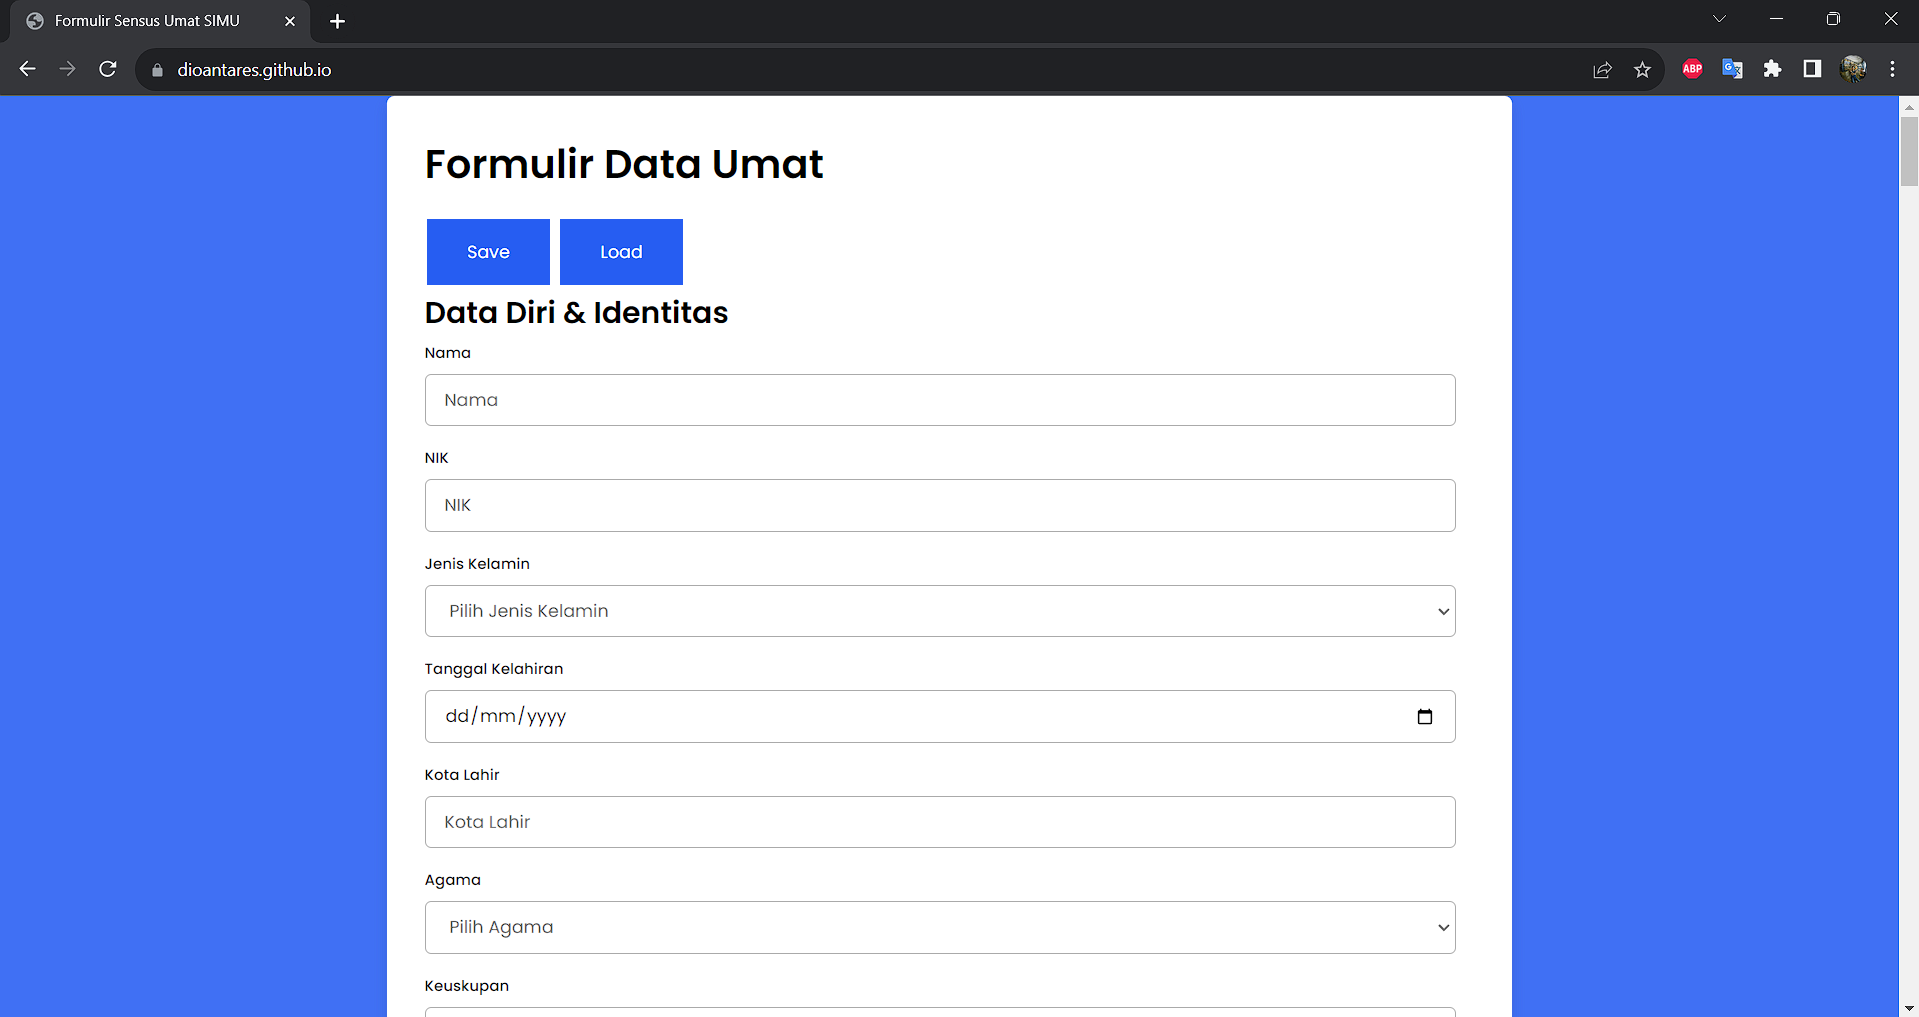
\includegraphics[scale=0.41]{Gambar/halamanFormulir.png}
	\caption{Rancangan antarmuka halaman Formulir Data Umat} 
	\label{fig:formDataUmatFull}
\end{figure}

\subsection{Tampilan Antarmuka Odoo}

\begin{figure}[H]
	\centering
	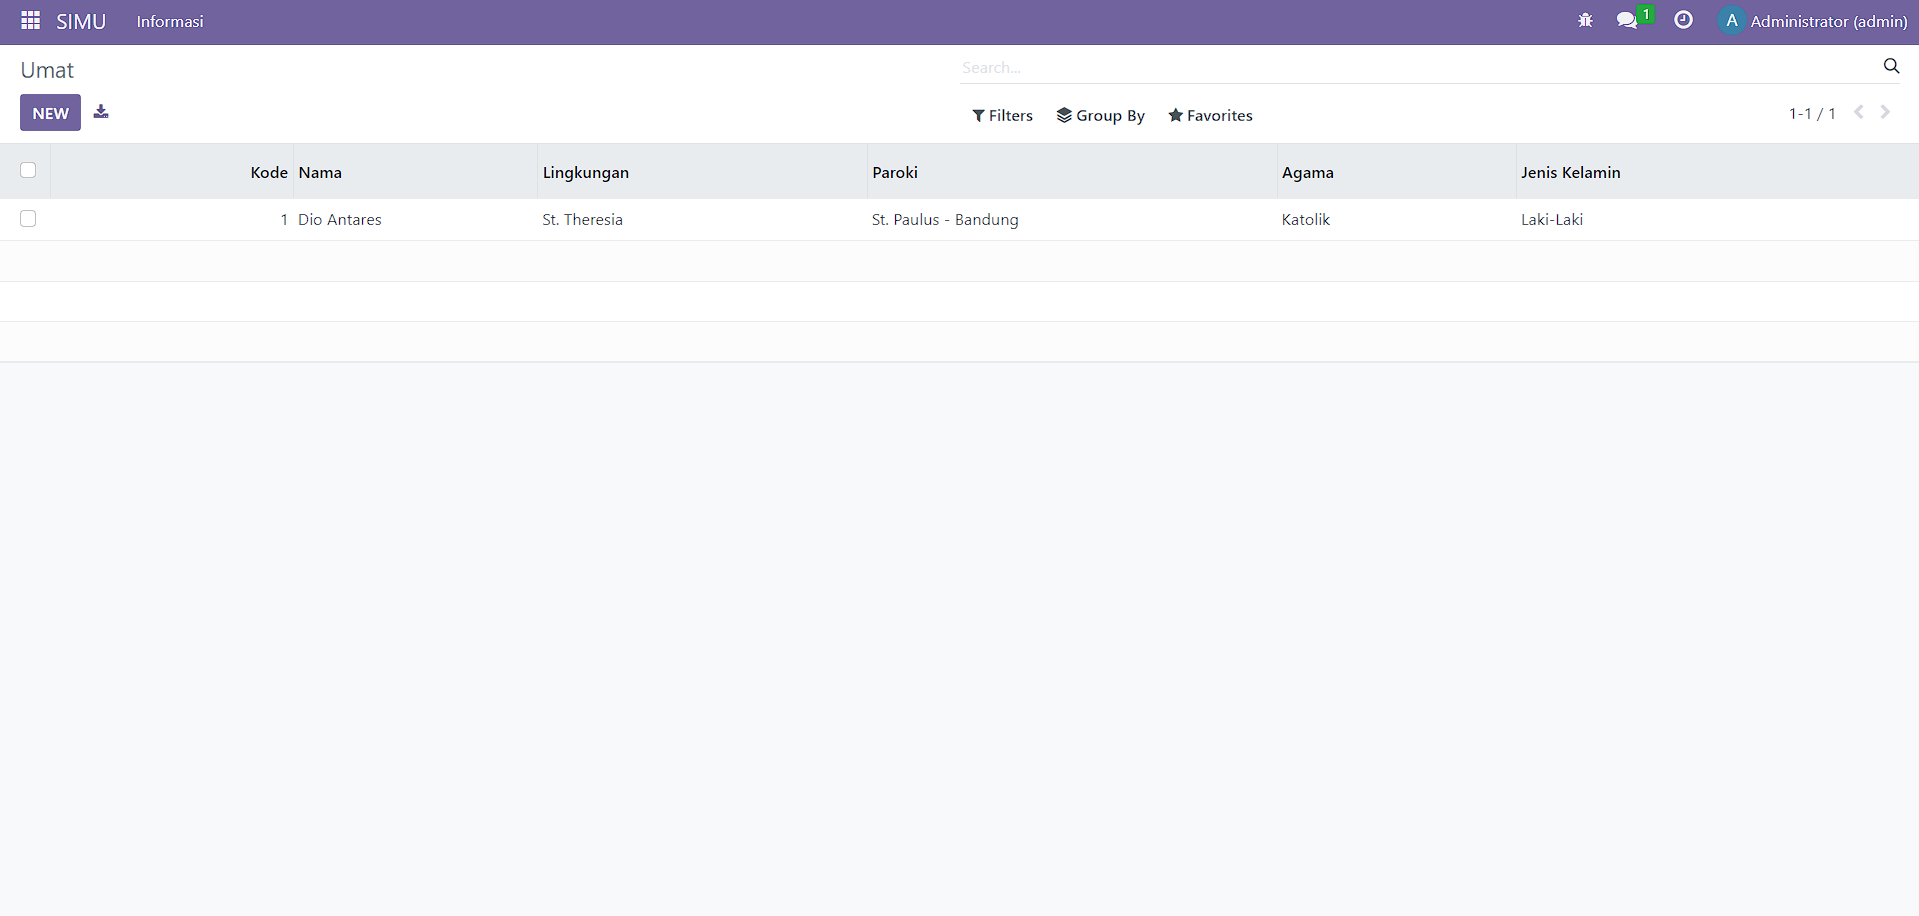
\includegraphics[scale=0.4]{Gambar/odooBuatBaru.png}
	\caption{Rancangan antarmuka halaman Odoo} 
	\label{fig:odooBuatBaru}
\end{figure}

\begin{figure}[H]
	\centering
	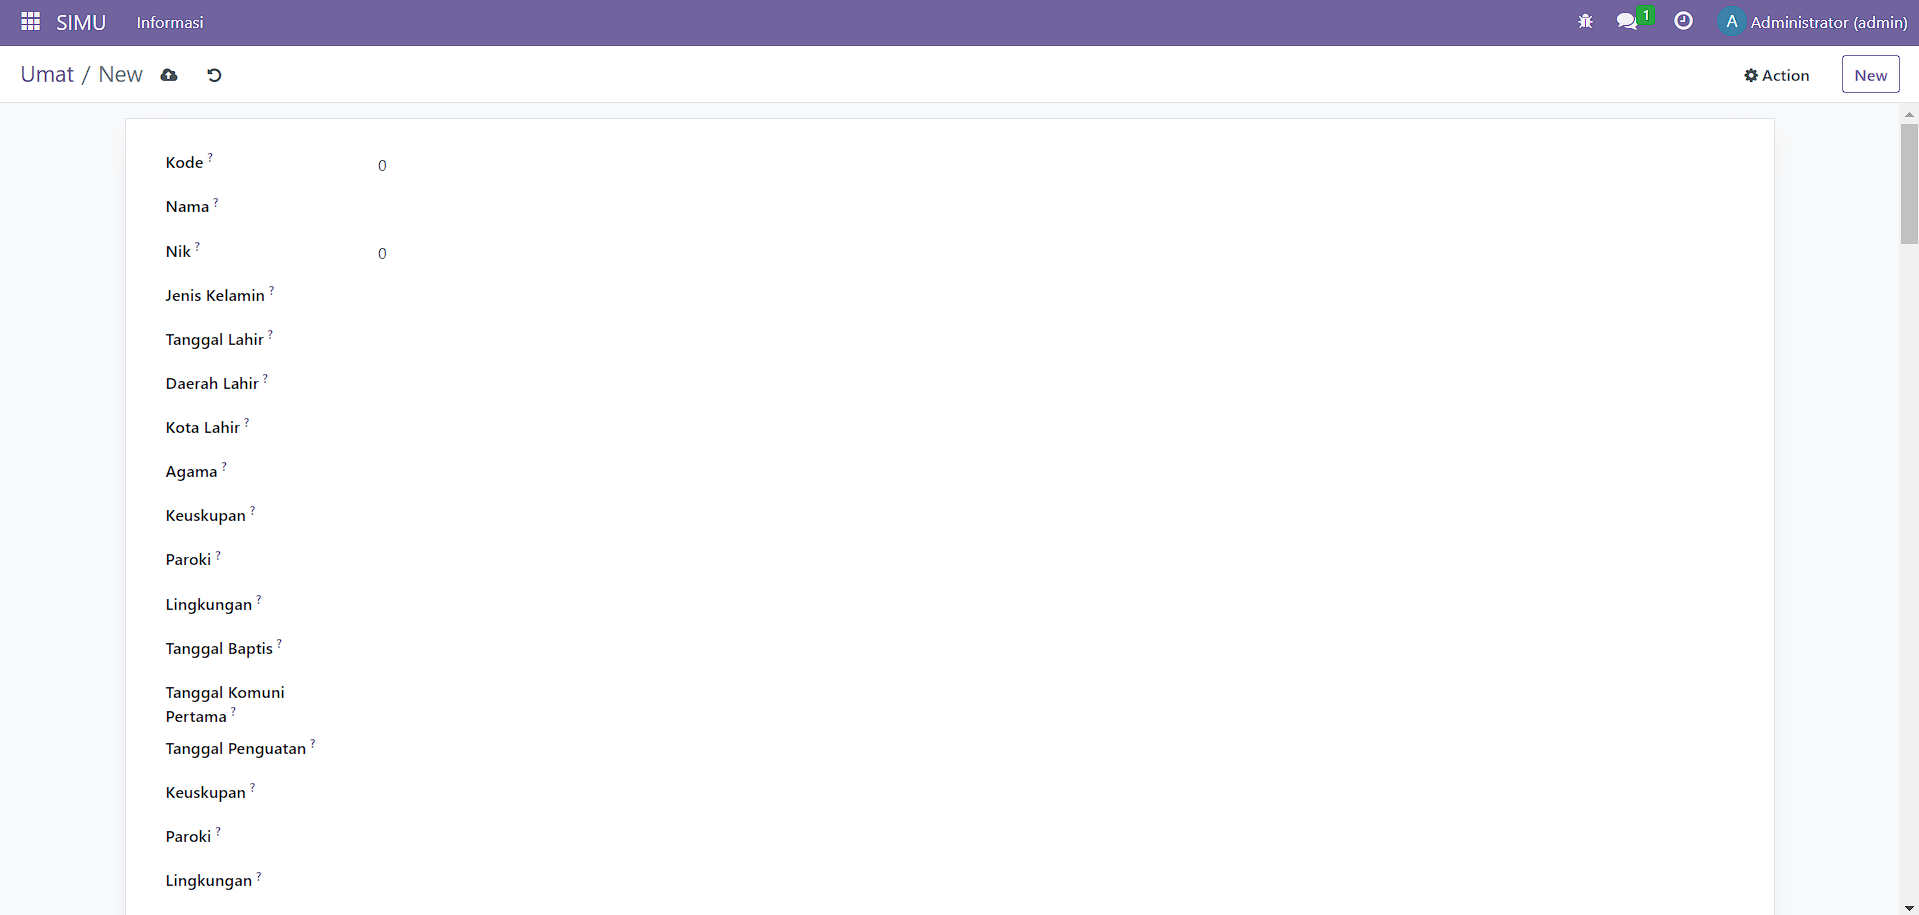
\includegraphics[scale=0.4]{Gambar/odooBuatBaru2.png}
	\caption{Rancangan antarmuka halaman Odoo} 
	\label{fig:odooBuatBaru2}
\end{figure}

Gambar \ref{fig:formDataUmatFull} merupakan tampilan antarmuka pada halaman Formulir Data Umat yang sudah diimplementasikan, sedangkan pada gambar \ref{fig:odooBuatBaru} merupakan halaman utama yang menampilkan data umat, lalu pada gambar \ref{fig:odooBuatBaru2} merupakan halaman odoo yang berfungsi untuk menambahkan data umat baru, untuk menuju halaman ini, admin perlu menakan tombol \textit{New} pada pojok kiri atas halaman utama.

\section{Pengujian Fungsional}
\label{sec:pengujianFungsional}

Pengujian fungsional dilakukan secara lokal pada perangkat penulis. Berikut ini pengujian yang dilakukan terhadap fitur-fitur yang sudah diimplementasi:

\subsection{Pengujian Fungsional Formulir Data Umat Baru}

\begin{table}[H]
	\centering
	\caption{Tabel Pengujian Fungsional Formulir Data Umat Baru}
	\begin{tabular}{|p{0.5cm}| p{5cm}| p{5.5cm}| p{2.5cm}|} \hline
		No.	&	Aksi Pengguna	&	Reaksi yang diharapkan	&	Reaksi \\ \hline
		1 	&  Membuka halaman utama & Halaman formulir ditampilkan &	sesuai	\\ \hline
		2 	&  Membuka halaman pada ponsel & Responsif (terbaca mudah di ponsel) &	sesuai	\\ \hline
		3 	&  Mengetik data pada form yang tersedia & Menampilkan keyboard yang tepat untuk input tertentu (contoh: nomor telepon menggunakan keypad) &	sesuai	\\ \hline
		4 	&  Menekan tombol save & Data disimpan ditandai dengan \textit{status} "Data Berhasil di Save" &	sesuai	\\ \hline
		5 	&  Menekan tombol Load & Data diload ditandai dengan \textit{status} "Data Berhasil di Load" &	sesuai	\\ \hline
		6 	&  Menekan tombol Submit & Menampilkan kode QR sesuai dengan data yang telah diisi &	sesuai	\\ \hline
	\end{tabular}
	\label{table:fungsionalFormulir}
\end{table}

\subsection{Pengujian Fungsional Odoo}

\begin{table}[H]
	\centering
	\caption{Tabel Pengujian Fungsional Odoo}
	\begin{tabular}{|p{0.5cm}| p{5cm}| p{5.5cm}| p{2.5cm}|} \hline
		No.	&	Aksi Pengguna	&	Reaksi yang diharapkan	&	Reaksi \\ \hline
		1 	&  Membuka halaman utama & Halaman utama ditampilkan &	sesuai	\\ \hline
		2 	&  Menekan tombol New & Menampilkan halaman dengan field data umat baru &	sesuai	\\ \hline
		3 	&  Menekan tombol Scan & Mampu memindai kode QR  &	belum sesuai	\\ \hline
	\end{tabular}
	\label{table:fungsionalOdoo}
\end{table}





